

%%% This LaTeX source document can be used as the basis for your technical
%%% report. Intentionally stripped and simplified
%%% and commands should be adjusted for your particular paper - title, 
%%% author, citations, equations, etc.
% % Citations/references are in report.bib 

\documentclass[conference,backref=page]{acmsiggraph}
\usepackage{dblfloatfix}
\usepackage[]{algorithm2e}
\usepackage{graphicx}
\usepackage{booktabs}
\usepackage{float}
\usepackage{listings}
\usepackage{color}

\definecolor{dkgreen}{rgb}{0,0.6,0}
\definecolor{gray}{rgb}{0.5,0.5,0.5}
\definecolor{mauve}{rgb}{0.58,0,0.82}

\lstset{frame=tb,
	language=Java,
	aboveskip=3mm,
	belowskip=3mm,
	showstringspaces=false,
	columns=flexible,
	basicstyle={\small\ttfamily},
	numbers=none,
	numberstyle=\tiny\color{gray},
	keywordstyle=\color{blue},
	commentstyle=\color{dkgreen},
	stringstyle=\color{mauve},
	breaklines=true,
	breakatwhitespace=true,
	tabsize=3
}


\TOGonlineid{45678}
\TOGvolume{0}
\TOGnumber{0}
\TOGarticleDOI{1111111.2222222}
\TOGprojectURL{}
\TOGvideoURL{}
\TOGdataURL{}
\TOGcodeURL{}

% Include this so that citations show up in blue and the page information is included in the reference section
\hypersetup{
    colorlinks = true, 
    linkcolor = blue,
    anchorcolor = red,
    citecolor = blue, 
    filecolor = red, 
}


\title{Solving The Travelling Salesman Problem\\
	   A Report Analysing the Algorithms Used}

\author{Beej Persson\thanks{e-mail:40183743@live.napier.ac.uk} \\
Edinburgh Napier University\\
Algorithms and Data Structures (SET09117)}
\pdfauthor{Beej Persson}

\keywords{algorithms, data structures, travelling salesman, efficacy, efficiency, problem solving.}

\begin{document}

\maketitle

\raggedbottom

\begin{abstract}

The Travelling Salesman Problem is a common algorithmic problem often discussed in computer science. The problem itself is to find the shortest route of travel between all the desired cities without going to a city twice. This report looks to analyse two algorithmic solutions to this problem and compare them against each other. The first solution is the Nearest Neighbour algorithm whilst the second is a modified and enhanced version of that algorithm. Multiple tests were run to evaluate their efficacy, including measuring run time, comparing route lengths and increasing the number of cities.

\end{abstract}

\keywordlist

\section{Introduction}

\paragraph{The Problem}
Given a list of cities and their locations (and therefore the distances between each city), what is the shortest route from a starting city that travels to each city only once before returning to the starting city? Solving this problem is often not only about achieving the shortest possible route, there is a focus on optimisation: finding this shortest route in a reasonable time given the number of cities.

\paragraph{First Solution: Nearest Neighbour Basic}
The Nearest Neighbour algorithm used here solves the problem by starting with the first city in the file, checking the distances between it and all the other cities, picking the shortest distance then doing the same for that closest city with all the rest, whilst removing each previous city. The pseudo-code for this algorithm is shown in Algorithm \ref{nnbasic}. This algorithm tends to return fairly short routes (although rarely the shortest) whilst also being fairly efficient. When used on a larger number of cities, the run time will still be comparatively low. This is due to it having an order of complexity of $n^2$, or $O(n^2)$, where the run time will increase in proportion to the problem size squared (for example the theoretical run time on a set of 10 cities will be 4 times bigger than on a set of 5, as $(10/5)^2 = 4$).

\begin{algorithm}[h]
	\KwData{Array List of unsorted cities}
	\KwResult{Empty Array List (for sorted cities)}
	Point2D closest = null\;
	Point2D currentCity = Data.get(0)\;
	\While{cities.size \textgreater 0}{
		add currentCity to Result\;
		remove currentCity from Data\;
		distance = infinity\;
		\For{all city in Data}{
			\If{getDistance(currentCity to city) \textless distance}{
				closest = city\;
				distance = getDistance(currentCity to city)\;
			}
		}
		currentCity = closest\;
	}
	return Result\;
	\caption{Nearest Neighbour Basic}
	\label{nnbasic}
\end{algorithm}

\paragraph{Second Solution: Nearest Neighbour Enhanced}
The Nearest Neighbour Enhanced algorithm uses a fairly simple adaptation to the previous algorithm. Instead of starting with the first city in the file, it will start with a random city and find the closest city to it and carry on from there. After that it will calculate the length of that route. It will do these two steps a number of times (specifically a tenth of the number of cities in the file) and then look over the list of lengths and pick the lowest route length found. The pseudo-code for this algorithm is shown in Algorithm \ref{nnenhanced}. This algorithm should consistently find lower route lengths at the expense of increased run time. As it is running the previous algorithm $n/10$ times (where n is the number of cities), its order of complexity is $O(n^3)$. This means that as the problem size increases, the run time will increase significantly (for example, the theoretical run time on a set of 10 cities will be 8 times bigger than on a set of 5, as $(10/5)^3 = 8$).

\begin{algorithm}[h]
	\KwData{Array List of unsorted cities}
	\KwResult{Empty Array List (for sorted cities)}
	Array List of Array Lists sortedCitiesList\;
	Array List lengths\;
	\For{int i \textless cities.size/10, i++}{
		Array List tempCitiesList = Data\;
		add nearestNeighbourRandomStart(tempCitiesList) to sortedCitiesList\;
		add routeLength(sortedCitiesList.get(i)) to legnths\;
		distance = infinity\;
		\If{lengths.get(i) \textless distance}{
			distance = lengths.get(i)\;
			Result = sortedCitiesList.get(i)\;
		}
	}
	return Result\;
	\caption{Nearest Neighbour Enhanced}
	\label{nnenhanced}
\end{algorithm}

\section{Experimental Method}

\paragraph{Overview}
The algorithms were tested against each other and on a variety of problem instances, with differing numbers of cities in each problem instance. The time it took the algorithm to return a sorted list of cities from the original unsorted list was used as the Run Time. The Route Length results were determined by calculating the length of the route between all the cities in the order of the sorted cities list. Tests were repeated for each algorithm for every problem instance. The results used in the later graphics were the averages of these repeated tests.

\paragraph{Detailed Description}
\begin{itemize}
\item {\bf Functionality of One Test}: Problem instance files containing a list of a certain number, $n$, of cities were loaded into an array list in Java. The algorithms sort this array list into an ordered list of cities, the order being the shortest route it found. The Run Time is calculated by finding the difference between the current time in milliseconds immediately before the algorithm is run and immediately after it returns a sorted list. This sorted list is then passed through a method that calculates the Route Length of the sorted cities in order. The Run Time and Route Length results were recorded for each test.
\item {\bf Testing Methodology}: For each of the chosen problem instances ten tests were run on each algorithm. For each test the results for the Run Time and the Route Length were then recorded in a table in an Excel file (see Figure \ref{exampletesttable}). The average Run Time and Route Length for each algorithm were stored in a separate table (Figure \ref{avgresultstable}) against the number of cities, $n$. This was the testing method used to produce the results and graphs analysed in this report.
\end{itemize}

\paragraph{Accuracy, Reliability and Reasoning for Testing Methodology}
 The number of cities in the file is initially known and is part of the file name. The number of cities in the array list (that the cities from the file are loaded into) is checked to match the number of cities in the file, and checked again after the algorithm is run. This is to ensure that the Route Length for the shortest route found is including every city in the problem instance and eliminate any artificially short routes. Nine problem instances were used, with an appropriately varying number of cities in each (ranging from 52 cities, up to 5915 cities) to help visualise the effect of $n$ on the Run Time of the two algorithms. Each problem instance tested stored the location of cities as points in Euclidean 2D geometry (with $x$, $y$ coordinates) and the way the software loaded the file's city list into an array list relied upon the city locations being stored this way. Therefore only problem instances that stored the cities in this way were tested. The Run Time results were recorded in milliseconds to best represent the time taken, with a problem instance with a small number of cities taking only a few milliseconds, and larger sample sizes taking hundreds and even thousands of milliseconds. Seconds could also have been chosen and been similarly effective due to the wide range of times achieved. The Route Length results were recorded with arbitrary units, as the location of each city was simply stored as a 2D point in the files with no indication of the units of the $x$ and $y$ coordinates. Each test was run on the same PC, from the same code, with each result being recorded one at a time to reduce memory build up slowing down Run Time and improve the accuracy and repeatability of the results. Ten tests were run for each problem instance and for each algorithm and the average Run Times and Route Lengths were used for displaying the results to further improve reliability of the accuracy of the testing methodology.


\section{Results}
Shown in this section are the results of the testing.

\begin{figure}[h]
	\begin{center}
		\resizebox{\columnwidth}{!}{%
		\begin{tabular}{@{}r|cccc@{}}
			\toprule
			\multicolumn{1}{l}{} & \multicolumn{4}{c}{u1060.tsp -\textgreater n = 1060} \\ \midrule
			\multicolumn{1}{l|}{} & \multicolumn{2}{c|}{Nearest Neighbour Basic} & \multicolumn{2}{c}{Nearest Neighbour Enhanced} \\ \midrule
			\multicolumn{1}{c|}{Test} & \multicolumn{1}{c|}{Time / ms} & \multicolumn{1}{c|}{Route Length / units} & \multicolumn{1}{c|}{Time / ms} & Route Length / units \\ \midrule
			1 & 13 & \multicolumn{1}{c|}{296,543.889} & 1,095 & 282,301.279 \\
			2 & 14 & \multicolumn{1}{c|}{296,543.889} & 1,104 & 281,639.607 \\
			3 & 13 & \multicolumn{1}{c|}{296,543.889} & 1,109 & 281,581.385 \\
			4 & 14 & \multicolumn{1}{c|}{296,543.889} & 1,103 & 281,006.855 \\
			5 & 13 & \multicolumn{1}{c|}{296,543.889} & 1,103 & 281,581.385 \\
			6 & 13 & \multicolumn{1}{c|}{296,543.889} & 1,103 & 281,006.855 \\
			7 & 13 & \multicolumn{1}{c|}{296,543.889} & 1,109 & 281,329.829 \\
			8 & 13 & \multicolumn{1}{c|}{296,543.889} & 1,093 & 281,444.456 \\
			9 & 14 & \multicolumn{1}{c|}{296,543.889} & 1,099 & 282,083.731 \\
			10 & 13 & \multicolumn{1}{c|}{296,543.889} & 1,106 & 281,329.829 \\ \midrule
			Avg & 13.3 & \multicolumn{1}{c|}{296,543.889} & 1,102.4 & 281,530.521 \\ \bottomrule
		\end{tabular}%
		}
		\caption{The table produced from the results of ten tests run for each algorithm on the file u1060.tsp, where $n$ is the number of cities which equals 1060.}
		\label{exampletesttable}
	\end{center}
\end{figure}

Figure \ref{exampletesttable} shows an example table of the testing. The problem instance file name and the number of cities in that file is at the top and the test number that the results correspond to are on the left. The results for both algorithms were stored in the same table in separate columns and the averages of the results are shown at the bottom of the table. The Run Time results were recorded to the nearest millisecond, whereas Route Length was to three decimal places. A table similar to this was produced for all nine problem instances and an averages table (see Figure \ref{avgresultstable}) was produced from the averages of the results from each test of the algorithms on the separate problem instances. For some comparisons made later, a ratios table (see Figure \ref{ratioresultstable}) was also produced by deriving the ratio of the Enhanced algorithm's results compared to the Basic algorithm's. Shown to the right is that final averages table.

\begin{figure}[h]
	\begin{center}
		\resizebox{\columnwidth}{!}{%
			\begin{tabular}{@{}rcccc@{}}
				\toprule
				\multicolumn{1}{l}{} & \multicolumn{4}{c}{Averages} \\ \midrule
				\multicolumn{1}{l|}{} & \multicolumn{2}{c|}{Nearest Neighbour Basic} & \multicolumn{2}{c}{Nearest Neighbour Enhanced} \\ \midrule
				\multicolumn{1}{c|}{n} & \multicolumn{1}{c|}{Time / ms} & \multicolumn{1}{c|}{Route Length / units} & \multicolumn{1}{c|}{Time / ms} & Route Length / units \\ \midrule
				\multicolumn{1}{r|}{52} & 0.6 & \multicolumn{1}{c|}{8,980.92} & 1.0 & 8,883.10 \\
				\multicolumn{1}{r|}{101} & 1.0 & \multicolumn{1}{c|}{825.24} & 2.5 & 759.50 \\
				\multicolumn{1}{r|}{159} & 1.6 & \multicolumn{1}{c|}{54,669.03} & 5.6 & 50,251.97 \\
				\multicolumn{1}{r|}{262} & 5.8 & \multicolumn{1}{c|}{3,241.47} & 19.9 & 2,920.33 \\
				\multicolumn{1}{r|}{493} & 4.9 & \multicolumn{1}{c|}{43,646.37} & 125.0 & 41,982.41 \\
				\multicolumn{1}{r|}{1060} & 13.3 & \multicolumn{1}{c|}{296,543.89} & 1,102.4 & 281,530.52 \\
				\multicolumn{1}{r|}{2103} & 44.2 & \multicolumn{1}{c|}{90,517.89} & 8,113.1 & 87,664.57 \\
				\multicolumn{1}{r|}{3795} & 137.1 & \multicolumn{1}{c|}{35,362.51} & 45,949.0 & 34,226.09 \\
				\multicolumn{1}{r|}{5915} & 336.4 & \multicolumn{1}{c|}{707,498.63} & 179,763.5 & 672,798.03 \\ \bottomrule
			\end{tabular}%
		}
		\caption{The Table of Averages produced by averaging all the results from the tests, where $n$ is the number of cities.}
		\label{avgresultstable}
	\end{center}
\end{figure}

The averages table has the problem instances' number of cities, $n$, on the left with the corresponding averages of the test results for each algorithm displayed in the neighbouring columns. The Run Times were recorded to one decimal place in milliseconds and the Route Length to the nearest two decimal places. This was to tidy the table up from the test tables.

\begin{figure}[h]
	\begin{center}
		\resizebox{\columnwidth}{!}{%
			\begin{tabular}{@{}rcccc@{}}
				\toprule
				\multicolumn{1}{l}{} & \multicolumn{4}{c}{Ratios} \\ \midrule
				\multicolumn{1}{l|}{} & \multicolumn{2}{c|}{Nearest Neighbour Basic} & \multicolumn{2}{c}{Nearest Neighbour Enhanced} \\ \midrule
				\multicolumn{1}{c|}{n} & \multicolumn{1}{l|}{Time / ms} & \multicolumn{1}{l|}{Route Length / units} & \multicolumn{1}{l|}{Time / ms} & \multicolumn{1}{l}{Route Length / units} \\ \midrule
				\multicolumn{1}{r|}{52} & 1.0 & \multicolumn{1}{c|}{1.0} & 1.7 & 0.989 \\
				\multicolumn{1}{r|}{101} & 1.0 & \multicolumn{1}{c|}{1.0} & 2.5 & 0.920 \\
				\multicolumn{1}{r|}{159} & 1.0 & \multicolumn{1}{c|}{1.0} & 3.5 & 0.919 \\
				\multicolumn{1}{r|}{262} & 1.0 & \multicolumn{1}{c|}{1.0} & 3.4 & 0.901 \\
				\multicolumn{1}{r|}{493} & 1.0 & \multicolumn{1}{c|}{1.0} & 25.5 & 0.962 \\
				\multicolumn{1}{r|}{1060} & 1.0 & \multicolumn{1}{c|}{1.0} & 82.9 & 0.949 \\
				\multicolumn{1}{r|}{2103} & 1.0 & \multicolumn{1}{c|}{1.0} & 183.6 & 0.968 \\
				\multicolumn{1}{r|}{3795} & 1.0 & \multicolumn{1}{c|}{1.0} & 335.1 & 0.968 \\
				\multicolumn{1}{r|}{5915} & 1.0 & \multicolumn{1}{c|}{1.0} & 534.4 & 0.951 \\ \bottomrule
			\end{tabular}%
		}
		\caption{The Table of Ratios shows how the Nearest Neighbour Enhanced algorithm compares to the Basic algorithm by seeing the results as a ratio of each other.}
		\label{ratioresultstable}
	\end{center}
\end{figure}

The ratios table has the problem instances' number of cities, $n$, on the left with the corresponding ratios for each algorithm displayed in the neighbouring columns. The Run Times and the Route Length results of both the Enhanced algorithm and the Basic algorithm were divided by the Basic algorithm's results to find the ratios shown.

\begin{figure*}[h]
	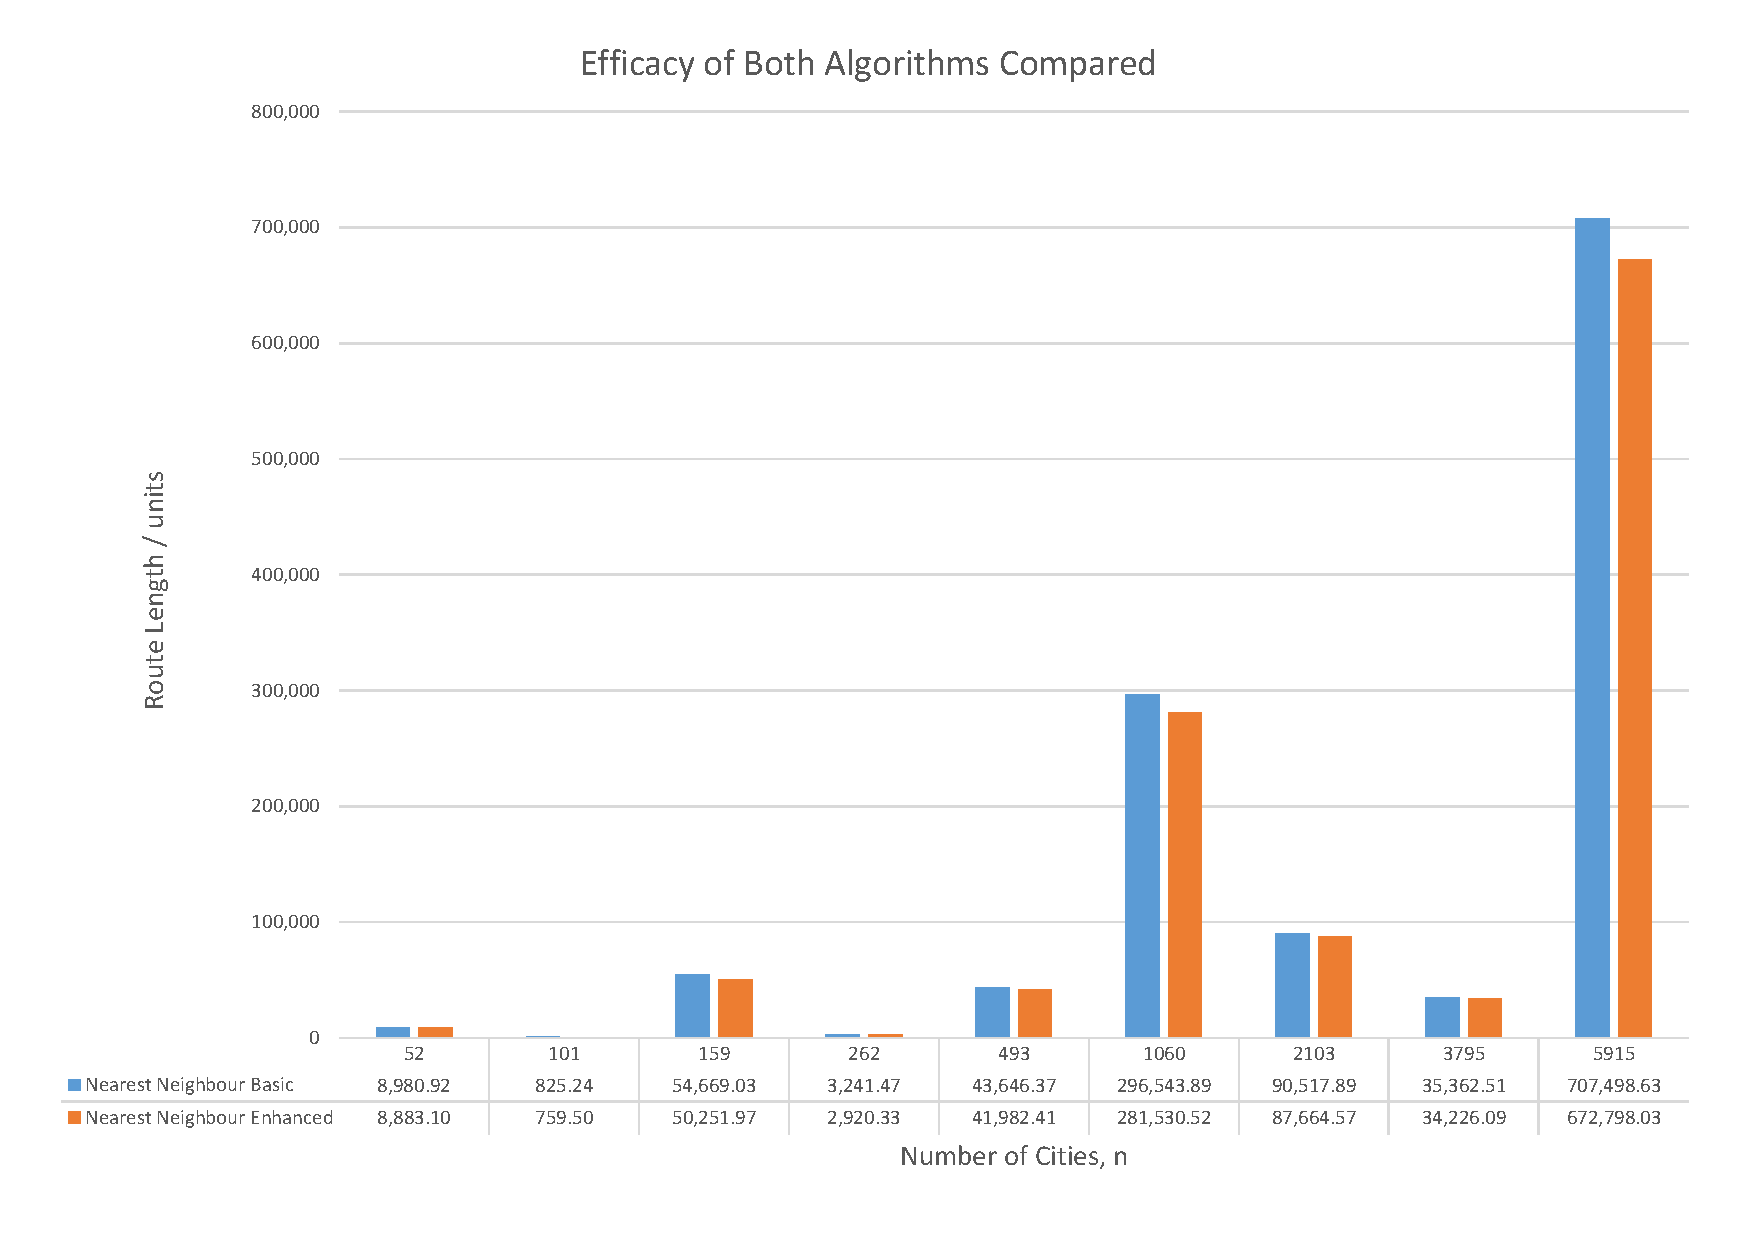
\includegraphics[width=\textwidth]{images/efficacy_compared.pdf}
	\caption{A graph showing the Nearest Neighbour Basic algorithm's average Route Length results compared against the Nearest Neighbour Enhanced algorithm's for the differing number of cities in each problem instance.}
	\label{efficacycomparedgraph}
\end{figure*}

\paragraph{Efficacy of Both Algorithms Compared}
The graph shown above (\ref{efficacycomparedgraph}) displays the results found for the Route Length for the shortest route found for both the Nearest Neighbour Basic and Nearest Neighbour Enhanced algorithms against the separate problem instances.

	
\begin{figure*}[h]
	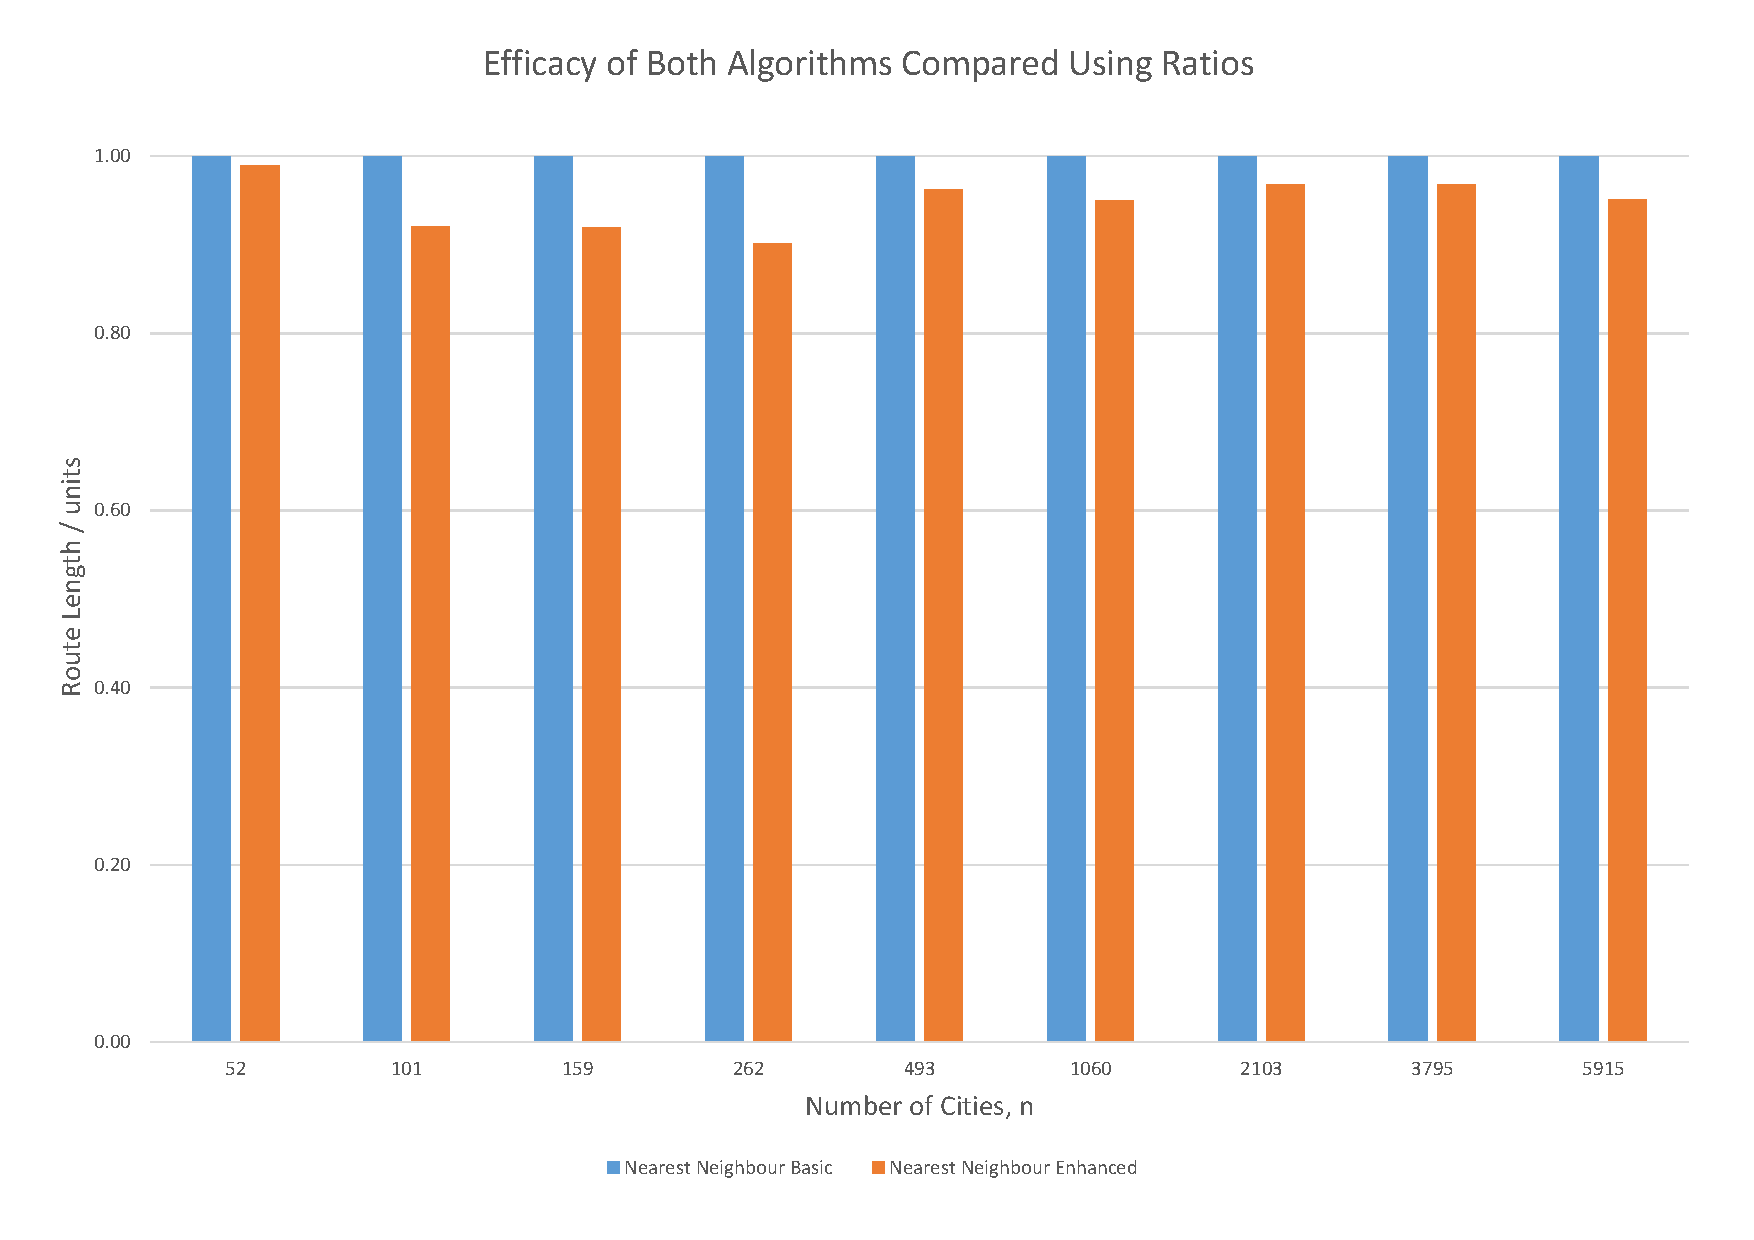
\includegraphics[width=\textwidth]{images/efficacy_compared_ratios.pdf}
	\caption{A graph showing the Nearest Neighbour Basic algorithm's average Route Length results compared against the Nearest Neighbour Enhanced algorithm's for the differing number of cities in each problem instance.}
	\label{efficacycomparedratiosgraph}
\end{figure*}

\begin{figure*}[h]
	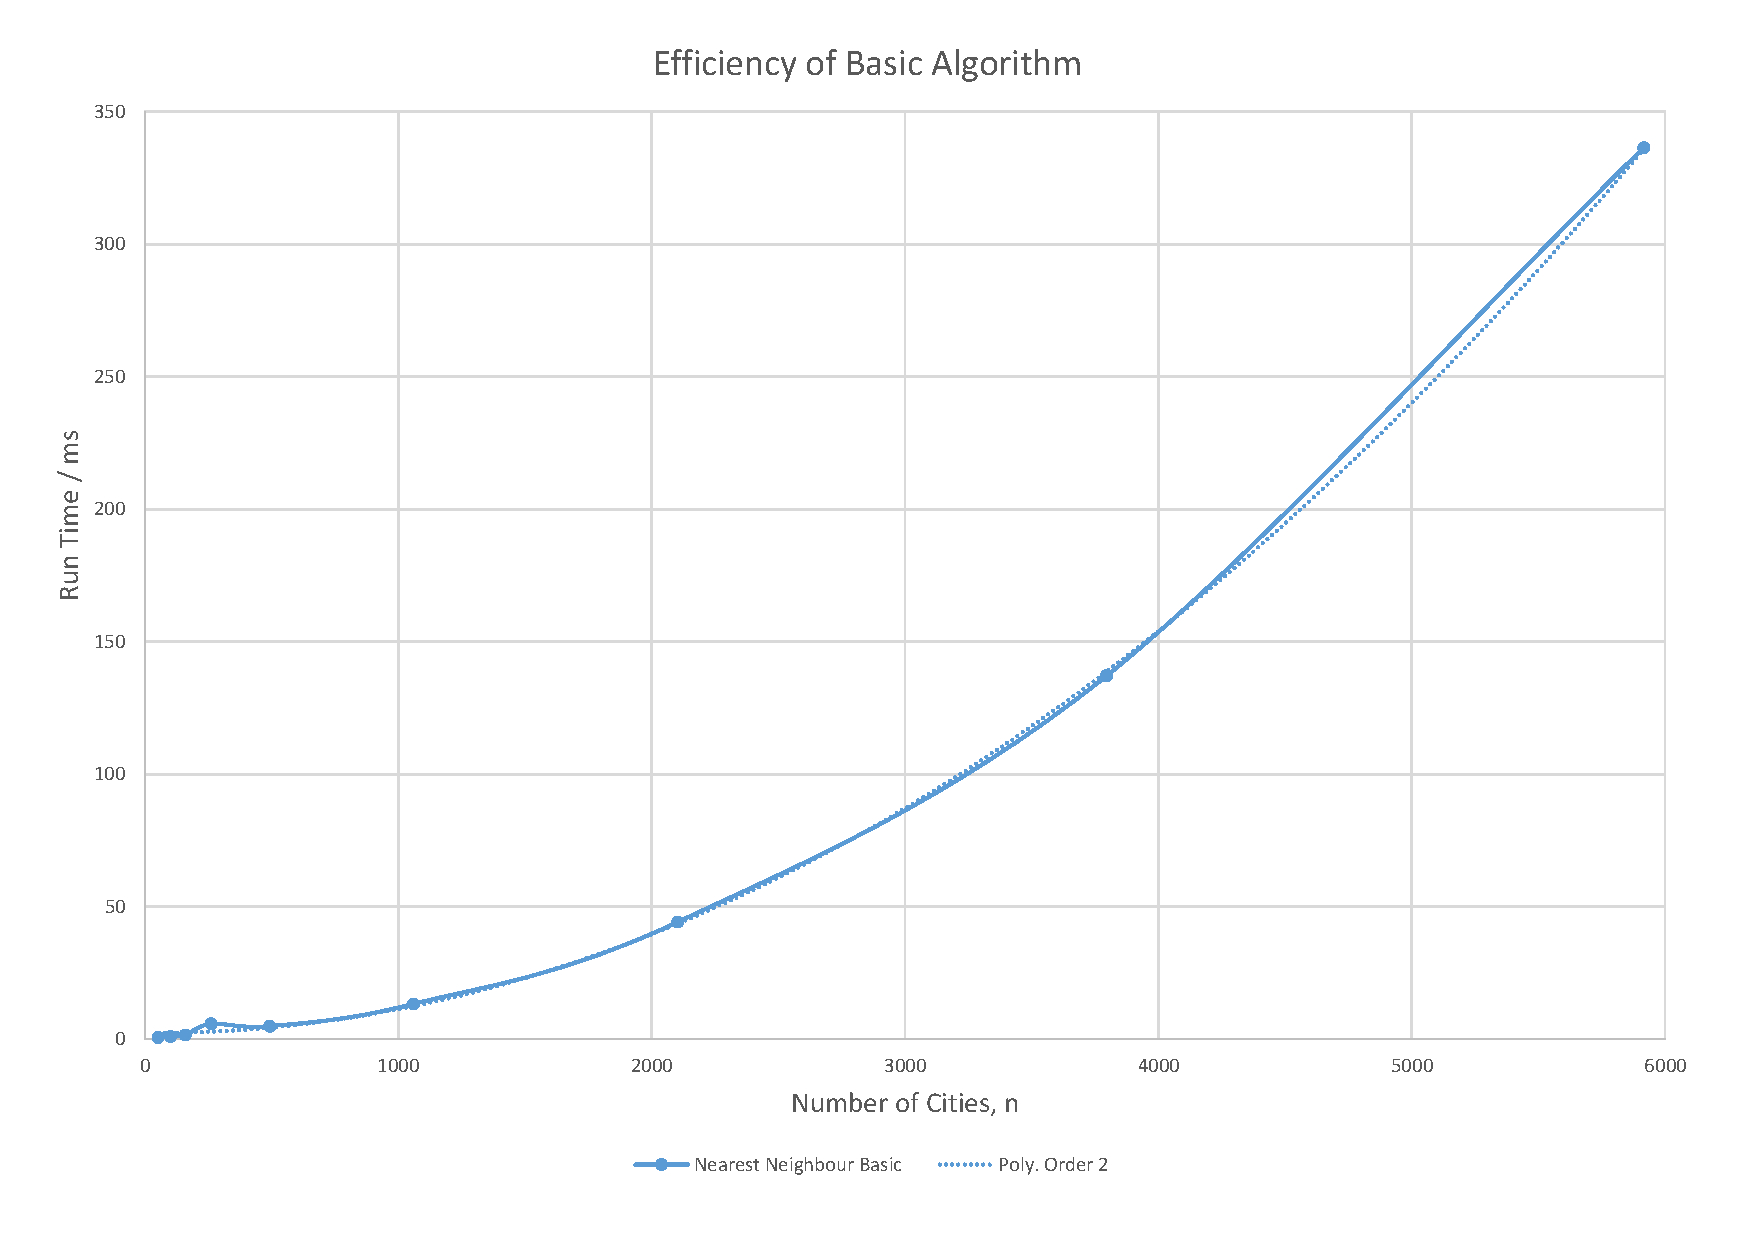
\includegraphics[width=\textwidth]{images/efficiency_basic.pdf}
	\caption{A graph showing the Nearest Neighbour Basic algorithm's average run time compared against the number of cities in each problem instance. The trendline is a polynomial trendline of order 2 aligning the algorithms order of complexity.}
	\label{efficiencybasicgraph}
\end{figure*}


\begin{figure*}[h]
	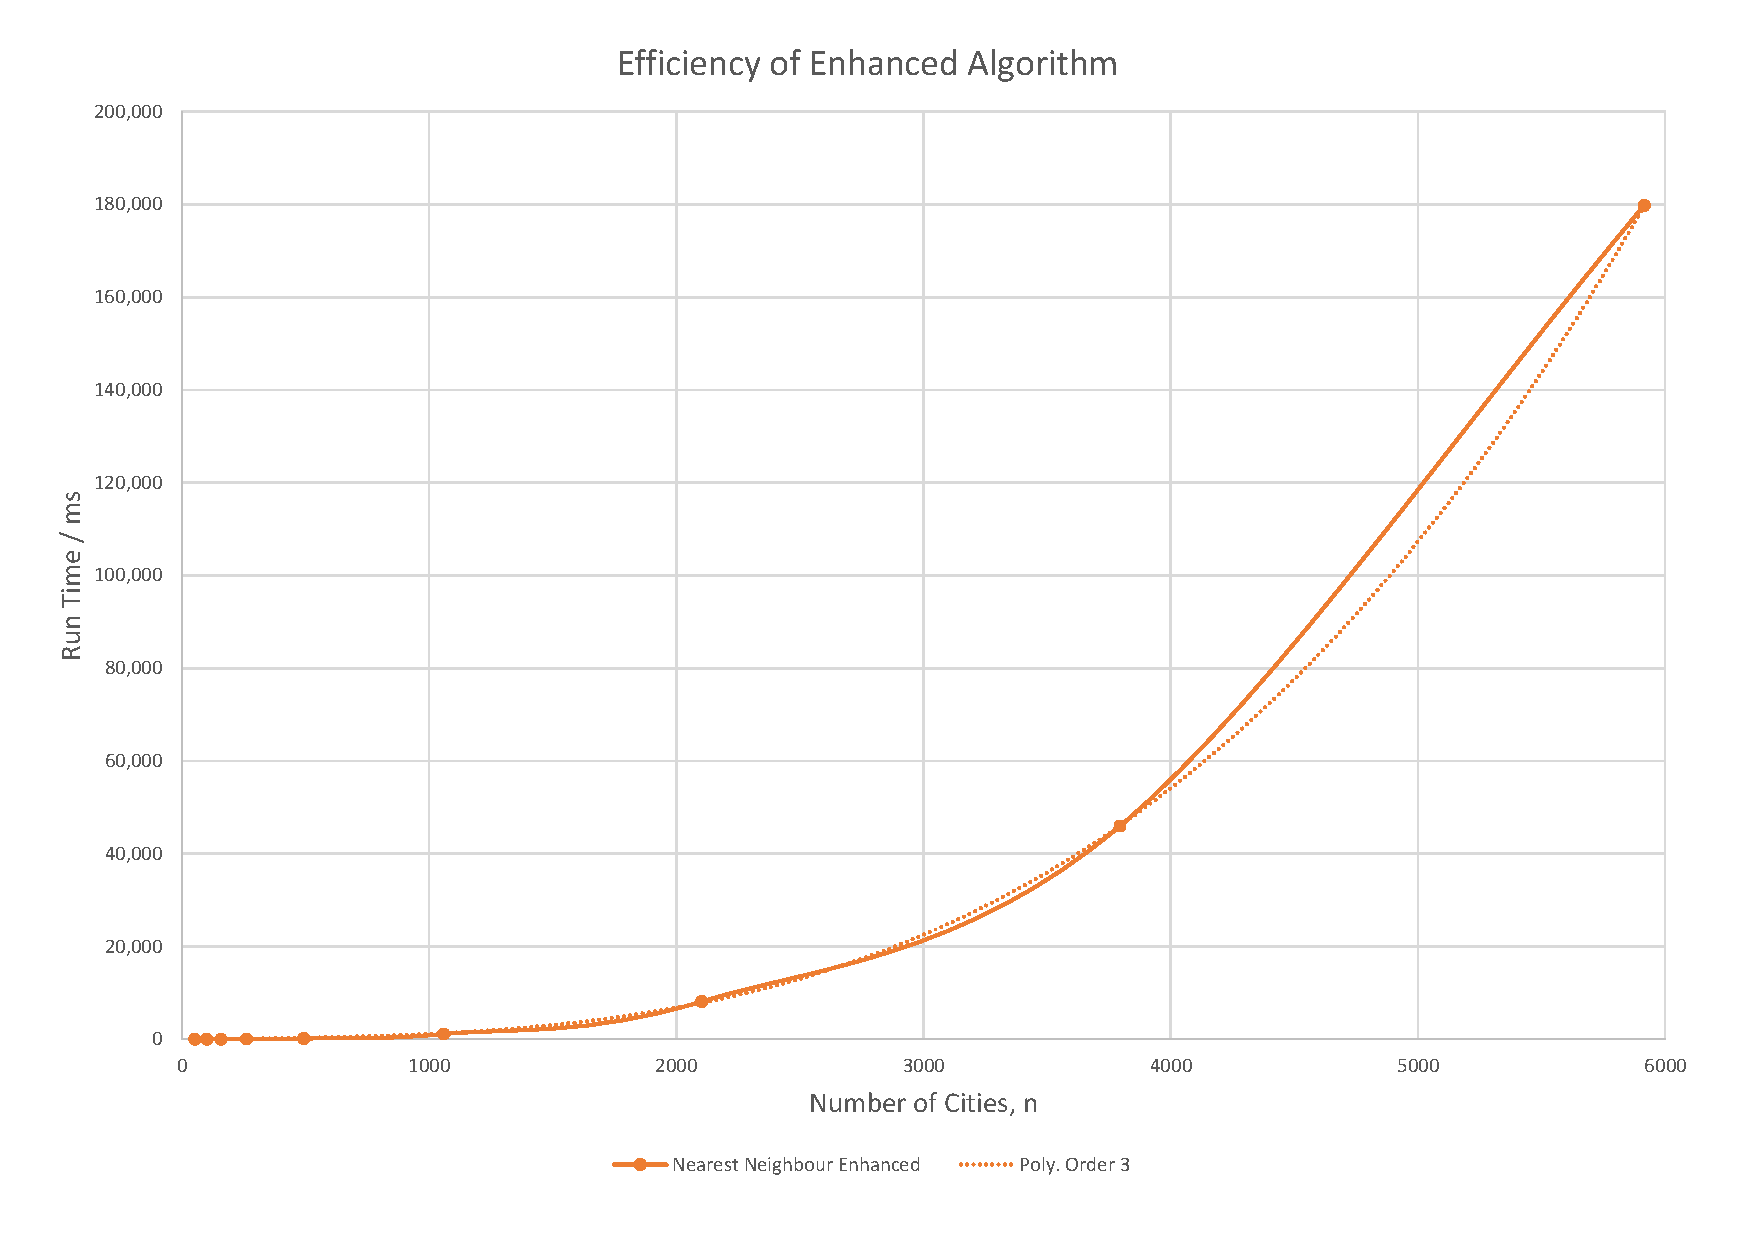
\includegraphics[width=\textwidth]{images/efficiency_enhanced.pdf}
	\caption{A graph showing the Nearest Neighbour Enhanced algorithm's average run time compared against the number of cities in each problem instance. The trendline is a polynomial trendline of order 3 aligning the algorithms order of complexity.}
	\label{efficiencyenhancedgraph}
\end{figure*}

\begin{figure*}[h]
	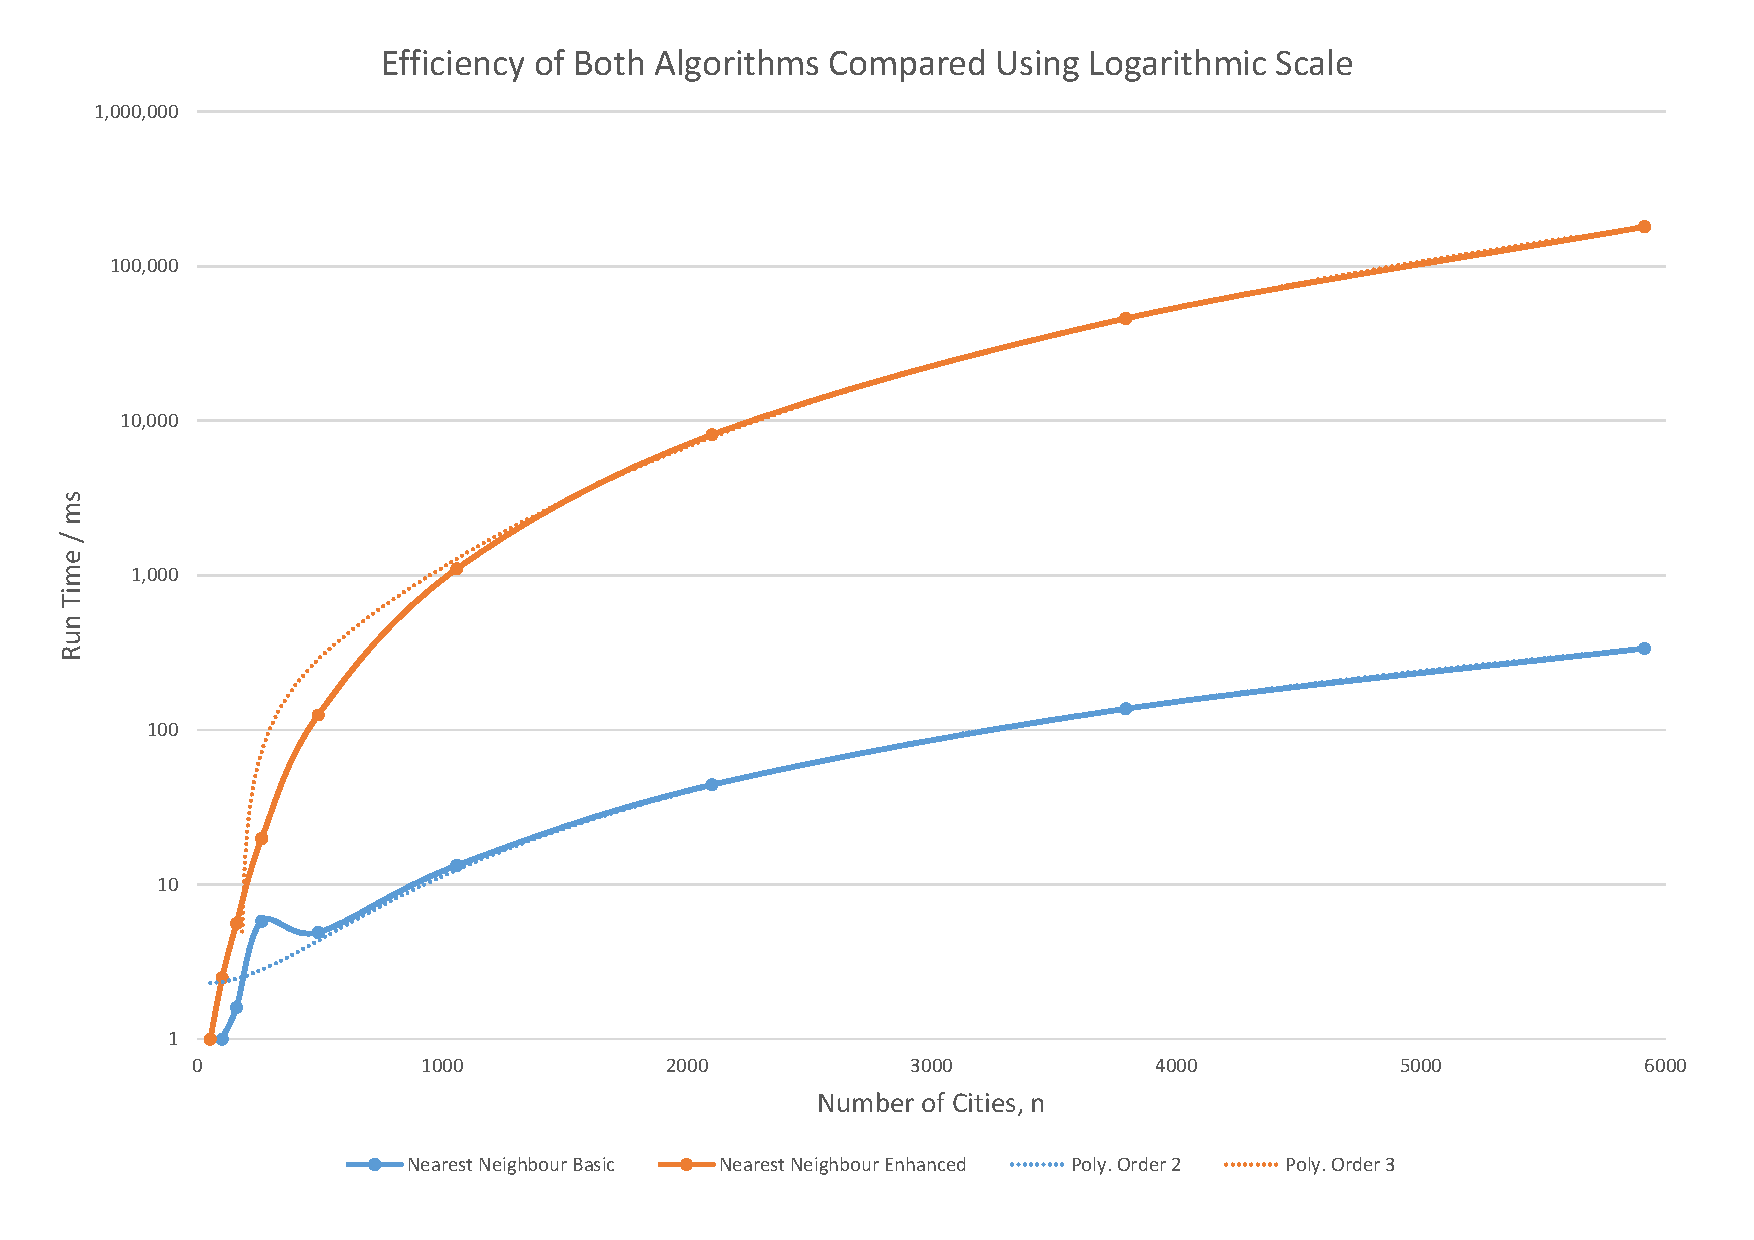
\includegraphics[width=\textwidth]{images/efficiency_compared.pdf}
	\caption{A graph showing the Nearest Neighbour Enhanced algorithm's average run time compared against the number of cities in each problem instance. The trendline is a polynomial trendline of order 3 aligning the algorithms order of complexity.}
	\label{efficiencycomparedgraph}
\end{figure*}

\clearpage
\section{Guidelines}
This section should be removed from your design report. Information provided here is to help you writing up your reports.

\begin{itemize}
\item Equations should be numbered and in the correct format, e.g., Equation \ref{eq:myequation} below:
\begin{equation} \label{eq:myequation}
 \sum_{j=1}^{z} j = \frac{z(z+1)}{2}
\end{equation}
\item Furthermore, if you include an equation, ensure you explain what each of the variables are (e.g., $F$ is force, $m$ is mass, and $a$ is the acceleration).
\item Don't using 'I' or 'Me'.
\item Each paragraph should be clear and focused, with multiple sentences that help make your point - avoid lots of single line paragraph sentence.
\item Make sure the citations are done using the correct formatting (i.e., .bib file and let LaTeX generate the references).
\item Every figure should have a caption, explaining what the picture is and what the reader should be looking at (i.e., what is important about the figure, what does it show)
\item A figure should also be referenced in the body of the main text (e.g., see Figure \ref{fig:teaser})
\item Equations should be numbered, and referenced in the text. Furthermore, ensure each of the variables in the equation are explained (i.e., don't use F=ma and not say what F, a, and m are)
\end{itemize}

\clearpage
\section{Appendix}

\textbf{Main.java}

\begin{lstlisting}

	import java.awt.geom.Point2D;
	import java.util.ArrayList;
	import java.util.Random;
	
	public class Main {
	
		public static double routeLength(ArrayList<Point2D> cities){
			//Calculate the length of a TSP route held in an ArrayList as a set of Points
			double result=0;//Holds the route length
			Point2D prev = cities.get(cities.size()-1);
			//Set the previous city to the last city in the ArrayList as we need to measure the length of the entire loop
			for(Point2D city : cities){
				//Go through each city in turn
				result += city.distance(prev);
				//get distance from the previous city
				prev = city;
				//current city will be the previous city next time
			}
			return result;
		}
		
		public static double getDistance(Point2D currentCity, Point2D possible){
		
			return Point2D.distance(currentCity.getX(), currentCity.getY(), possible.getX(), possible.getY());
		}
		
		public static ArrayList<Point2D> nearestNeighbourBasic(ArrayList<Point2D> cities){
			ArrayList<Point2D> result = new ArrayList<Point2D>();
			Point2D closest = null;
			Point2D currentCity = cities.get(0);
			while (cities.size() > 0){
				result.add(currentCity);
				cities.remove(currentCity);
				double distance = Double.POSITIVE_INFINITY;
				for (Point2D city : cities){
					if (getDistance(currentCity, city) < distance){
						closest = city;
						distance = getDistance(currentCity, city);
					}
				}
				currentCity = closest;
			}
			return result;
		}
		
		public static ArrayList<Point2D> nearestNeighbourRandomStart(ArrayList<Point2D> cities){
			ArrayList<Point2D> result = new ArrayList<Point2D>();
			Point2D closest = null;
			Random rn = new Random();
			int random = rn.nextInt(cities.size() + 1);
			Point2D currentCity = cities.get(random);
			while (cities.size() > 0){
				result.add(currentCity);
				cities.remove(currentCity);
				double distance = Double.POSITIVE_INFINITY;
				for (Point2D city : cities){
					if (getDistance(currentCity, city) < distance){
						closest = city;
						distance = getDistance(currentCity, city);
					}
				}
				currentCity = closest;
			}	
			return result;
		}
		
		public static ArrayList<Point2D> nearestNeighbourEnhanced(ArrayList<Point2D> cities){
			ArrayList<Point2D> result = new ArrayList<Point2D>();
			ArrayList<ArrayList<Point2D>> sortedCitiesList = new ArrayList<ArrayList<Point2D>>();
			ArrayList<Double> lengths = new ArrayList<Double>();
			for (int i = 0; i < (cities.size()/10); i++){
				ArrayList<Point2D> tempCitiesList = new ArrayList<Point2D>(cities);
				sortedCitiesList.add(nearestNeighbourRandomStart(tempCitiesList));
				lengths.add(routeLength(sortedCitiesList.get(i)));
				//System.out.println("Length of route: " + lengths.get(i));
				double distance = Double.POSITIVE_INFINITY;
				if (lengths.get(i) < distance){
					distance = lengths.get(i);
					result = sortedCitiesList.get(i);
				}
			}
			//System.out.println(distance);
			return result;
		}
		
		public static void main(String[] args) {
			//Loads in desired city file
			ArrayList<Point2D> cities = LibLoader.loadTSPLib("berlin52.tsp");
			//ArrayList<Point2D> cities = LibLoader.loadTSPLib("eil101.tsp");
			//ArrayList<Point2D> cities = LibLoader.loadTSPLib("u159.tsp");
			//ArrayList<Point2D> cities = LibLoader.loadTSPLib("gil262.tsp");
			//ArrayList<Point2D> cities = LibLoader.loadTSPLib("d493.tsp");
			//ArrayList<Point2D> cities = LibLoader.loadTSPLib("u1060.tsp");
			//ArrayList<Point2D> cities = LibLoader.loadTSPLib("d2103.tsp");
			//ArrayList<Point2D> cities = LibLoader.loadTSPLib("fl3795.tsp");
			//ArrayList<Point2D> cities = LibLoader.loadTSPLib("rl5915.tsp");
			
			//Print the number of cities for the file
			System.out.println("Number of cities in file: " + cities.size());
			
			// Start recording times
			final long startTime = System.currentTimeMillis();
			
			//Choose algorithm
			//ArrayList<Point2D> sortedCities = nearestNeighbourBasic(cities);
			ArrayList<Point2D> sortedCities = nearestNeighbourEnhanced(cities);
			
			//End recording time
			final long endTime = System.currentTimeMillis();			
			
			//Measure length of route found
			double length = routeLength(sortedCities);
			
			//Print results
			System.out.println("Route Length: " + length + "\nRun Time: " + (endTime - startTime) + "ms");
			
			//Print the number of cities for the file after the algorithm is run
			System.out.println("Number of cities in route: " + sortedCities.size());
		}
	}
\end{lstlisting}

\clearpage
\textbf{LibLoader.java}

\begin{lstlisting}

	import java.awt.geom.Point2D;
	import java.io.BufferedReader;
	import java.io.FileReader;
	import java.io.IOException;
	import java.util.ArrayList;
	
	public class LibLoader {
		
		public static ArrayList<Point2D> loadTSPLib(String fName){
			//Load in a TSPLib instance. This example assumes that the Edge weight type is EUC_2D.
			ArrayList<Point2D> result = new ArrayList<Point2D>();
			BufferedReader br = null;
			try {
				String currentLine;
				int dimension =0;//Hold the dimension of the problem
				boolean readingNodes = false;
				br = new BufferedReader(new FileReader(fName));
				while ((currentLine = br.readLine()) != null) {
					//Read the file until the end;
					if (currentLine.contains("EOF")){
						//EOF should be the last line
						readingNodes = false;
						//Finished reading nodes
						if (result.size() != dimension){
							//Check to see if the expected number of cities have been loaded
							System.out.println("Error loading cities");
							System.exit(-1);
						}
					}
					if (readingNodes){
						//If reading in the node data
						String[] tokens = currentLine.split(" ");
						//Split the line by spaces.
						//tokens[0] is the city id and not needed in this example
						float x = Float.parseFloat(tokens[1].trim());
						float y = Float.parseFloat(tokens[2].trim());
						//Use Java's built in Point2D type to hold a city
						Point2D city = new Point2D.Float(x,y);
						//Add this city into the arraylist
						result.add(city);
					}
					if (currentLine.contains("DIMENSION")){
						//Note the expected problem dimension (number of cities)
						String[] tokens = currentLine.split(":");
						dimension = Integer.parseInt(tokens[1].trim());
					}
					if (currentLine.contains("NODE_COORD_SECTION")){
						//Node data follows this line
						readingNodes = true;
					}
				}
			} catch (IOException e) {
			e.printStackTrace();
			} finally {
				try {
					if (br != null)br.close();
					} catch (IOException ex) {
					ex.printStackTrace();
					}
			}
			return result;
		}
	}
\end{lstlisting}


\end{document}

